\chapter{Methods}

\section{Data acquisition and mapping}

We have constructed an spectral integrated data acquisition and mapping system,
consisting of a Bridgeport Instruments cesium iodide scintillator detector, GPS
interface, and Windows laptop. Spectral data is recorded into a
PostGIS\cite{postgis} database on the laptop, along with each observation's GPS
location and timestamp.

\subsection{Scintillator interface}

The Bridgeport Instruments scintillator connects to the laptop via a simple USB
interface, with drivers provided by Bridgeport. A simple C API is provided with
documentation, allowing users to control the scintillator's high voltage power
supply, photomultiplier tube settings, and integrated multichannel
analyzer. Because our data analysis code was written in Python, it was necessary
to write a Python C extension which allows Python code to interface with the
detector.

The resulting \texttt{emorpho\_cpython} module is available at
\url{https://github.com/capnrefsmmat/emorpho-cpython}. It allows Python code to
connect to a scintillator detector over USB, alter its voltage and gain
settings, and collect either histograms or raw lists of counts. Statistics, such
as detector temperature, runtime and count rates, can be read off of the
device. The result is much easier to use than the raw C interface. The module is
compatible with Python 2.7.

\subsection{Recording of spectra}

The recording, analysis and mapping code is available online at
\url{https://github.com/capnrefsmmat/radmonitor}. Spectra were recorded at
two-second intervals by the monitoring code, along with the most recent
latitude, longitude and altitude provided by the GPS unit. These data were saved
in the PostGIS database along with detector temperature, estimated GPS
horizontal dilution of precision, current time, and gamma count rate.

Occasionally the GPS signal would be lost due to overhead obstructions. In these
cases, the system continues to record spectra, but without an attached location;
it is hoped that future work will allow these locations to be interpolated from
those recorded just prior to signal loss.

The monitoring system also runs a local webserver. Browsers viewing
\texttt{http://localhost:8080} are presented with a real-time graph of current
count rates and GPS precision, along with detector temperature and other
diagnostic data. This display was made available over a WiFi connection so the
detector could be monitored in real-time via smartphone, and was successfully
used to collect several hours of data.

\subsection{Mapping}

We used the \texttt{matplotlib}\cite{Hunter:2007} library for Python, along with
the Basemap Toolkit, to perform graphical mapping. During analysis, GPS latitude
and longitude coordinates were converted by PostGIS to the NAD83 (NSRS2007)
Texas Central (SRID 3663) coordinate system, a Lambert Conic Conformal
projection suitable for use in central Texas.\cite{nad83} All units are in
meters. This was substantially easier than working in latitude and longitude,
allowing observations to be placed on a Euclidean plane rather than a spheroid.

For reference, maps were plotted on top of OpenStreetMaps data of the local
area, including local building outlines and streets.\cite{osm} Observed count
rates were plotted as hexagonally-binned chloropleth maps. Spectral analysis was
done on square spatial bins, with each bin plotted with a color indicating the
spectra difference observed.

\section{Spectral comparison ratio anomaly detection}

The final component of the SCRAM system is our spectral anomaly detection
algorithm. This does not detect changes in radiation levels, but instead
examines spectral shapes. SCR collects observed gamma counts into energy bins,
which may be chosen to cover certain spectral regions of interest or can be
distributed evenly across the spectrum. Various methods exist to choose energy
bins targeted for detection of particular
isotopes;\cite{Wei:2010go,Pfund:2010hm} however, for this demonstration, we
simply chose 8 energy bins which contained roughly equal numbers of counts in a
typical background spectrum, covering the energy range between 100 and 2500 keV.

Binning the data into \(n\)
bins creates a vector of counts \(\mathbf{c} = [ c_1 c_2 \ldots c_n]\). We also
have a background vector, \(\mathbf{b}\), containing the mean observed spectrum
across all background observations, binned in the same way.  One energy bin is
chosen as the reference bin (in this case, bin 1). The choice of reference bin
is unimportant, as the anomaly statistic is invariant to the choice of bin
\cite{Runkle:2009ev}. The spectral comparison ratios can then be computed by:
\begin{equation}\label{scr}
s_i = c_1 - \frac{b_1}{b_i} c_i,
\end{equation}
for \(i > 1\). This is mathematically equivalent to multiplying the vector
\(\mathbf{c}\) by a spectral shape matrix \(S\):

\begin{equation}
S = \begin{pmatrix}
1 & - \frac{b_1}{b_2} & 0 & \ldots & 0 \\
1 & 0 & - \frac{b_1}{b_3} & \ldots & 0\\
\vdots \\
1 & 0 & 0 & \ldots & -\frac{b_1}{b_n} \\
\end{pmatrix}
\end{equation}

\begin{equation}
\mathbf{s} = S \cdot \mathbf{c}
\end{equation}

There are \((n - 1)\) linearly independent SCRs, since one bin is a reference
bin.  The SCR process compares \(c_1\) against projections based on the ratio
between bins in the background data and the counts in bin \(i\); the deviations
of the projections are given in the SCR vector \(\mathbf{s}\).  Since
\(\mathbf{s}\) is computed using ratios between bins, it is insensitive to
global changes in count rate unless they alter the spectral shape.  This
important feature allows for comparisons of spectra made with unequal
observation times.

With these useful properties, the SCR vector can be used to detect
\textit{spectral anomalies} based upon sound statistics, assuming an underlying
Poisson distribution.  Additionally, the statistical formulation allows for a
quantitative comparison between an observation's spectrum and previously
recorded observations.

\subsection{Characterizing expected variation}

To accurately detect anomalies, we first need to determine what variation can be
expected in the natural background. First, we assume that counts in each energy
bin are roughly Poisson-distributed. This would imply that the variance of the
count rate in a region is equal to its mean, which is not true in larger spatial
regions, as count rates become overdispersed. (See
Fig.~\ref{poisson-dispersion}). Consequently, we approximate that \(\text{var}
(c_i) = V c_i\), where \(V\) is the average variance-to-mean ratio of count
rates (\(V=1\) for perfectly Poisson-distributed counts). We know the
relationship between the variance of random variables:
\begin{equation}
\text{var}(aX + bY) =
a^2 \text{var}(X)  + b^2 \text{var}(Y) +  2 ab\, \text{cov}(X,Y)
\end{equation}

Hence, using (\ref{scr}) we may estimate \(\text{var}(s_i)\):

\begin{equation}
  \text{var}(s_i) = V c_1 + \left(\frac{b_1}{b_i}\right)^2 V c_i - 2
  \frac{b_1}{b_i} \text{cov}(c_1, c_i)
\end{equation}

The covariance \(\text{cov}(c_1, c_i)\) would ideally be estimated from all
previous background observations made in a spatial bin, so that
\(\text{cov}(c_1, c_i) \propto \text{cov}(b_1, b_i)\). However, spatial mapping
would be impractical if it required numerous repeated observations before
detecting anomalies. The relationship between the covariance \(\text{cov}(b_i,
b_j)\) and the correlation \(\text{corr}(b_i, b_j)\) is \cite{Morrison}:

\begin{equation}
  \text{cov}(b_i, b_j) = \text{corr}(b_i, b_j) \sqrt{\text{var}(b_i) \, \text{var}(b_j)}.
\end{equation}

To replace \(\text{cov}(c_1, c_i)\) with this we must also rescale;
\(\mathbf{b}\) may have resulted from an observation of a different length than
\(\mathbf{c}\). Consequently, we can replace the covariance with a correlation:
\begin{equation}\label{vars}
  \text{var}(s_i) = 
  V\left(c_1 + \left(\frac{b_1}{b_i}\right)^2 c_i - 2 \frac{b_1}{b_i}
  \left(\frac{T_c}{T_b}\right)^2 \text{corr}(b_1, b_i) \sqrt{b_1 b_i}\right),
\end{equation}
where \(T_c\) is the time taken to observe \(\mathbf{c}\) and \(T_b\) the time
taken to observe \(\mathbf{b}\). This is obtained by replacing
\(\text{var}(b_i)\) with \(\text{var}(b_i T_c/T_b)\), and likewise for \(\text{var}(b_j)\).

To compute \(\text{corr}(b_1,b_i)\) we do not rely only on background
observations made in the chosen spatial bin, as there is frequently not enough
data to make this possible. Instead, \(\text{corr}(b_1,b_i)\) is estimated from
observations in all bins by summing together observations into thirty-second
intervals. The correlation between bins in these summed observations is easily
computed.

Finally, we can compute the covariance matrix \(\Sigma\) between bins in the SCR
vector:
\begin{equation}
\Sigma_{ij} = \text{corr} (s_i, s_j) \sqrt{\text{var}(s_i) \text{var}(s_j)},
\end{equation}
where \(\text{corr} (s_i, s_j)\) is estimated by summing all observations across
all spatial bins in the same way as for \(\text{corr}(b_i,b_1)\), then comparing
each observation to the global mean spectrum to produce \(\mathbf{s}\).

% This following paragraph should be more convincing. -- 
% no kidding.

By using correlation matrices we have produced an anomaly detection method that
performs well with few past observations. Because the correlation matrices are
produced using all background observations, rather than only observations made
in a particular spatial region, there are sufficient observations for
well-conditioned and invertible matrices. A simpler method may be to directly
compute the covariance matrix in a single spatial bin, but this is only
practical if there are numerous observations, requiring repeated mapping passes;
covariance matrices are frequently singular or ill-conditioned
otherwise. Approaches based on shrinkage estimators are possible
\cite{Daniels:2001et}, but cannot work if there are only one or two
observations.

The correlation matrices may be computed and reused for anomaly detection in all
spatial bins; any similar method using covariance matrices would require each
spatial bin to contain observations of equal length each day, or require new
covariance matrices to be computed for each spatial bin. 

This method does rest on several assumptions; namely, gamma-ray counts must be
roughly Poisson-distributed, and the typical spectral variance should be roughly
the same over the entire region. When these assumptions are violated, the
resulting covariance matrices are likely too inaccurate to be of value.

\subsection{Anomaly detection}

Previous work has developed a simple anomaly detection algorithm which makes use
of the SCR vector \(\mathbf{s}\) \cite{Pfund:2007}. In these applications a set
of many independent background observations \(\mathbf{b}\) are made, and
\(\mathbf{s}\) is calculated for each observation. After computing the
covariance matrix \(\Sigma\) for the resulting set of SCR vectors,
\(\mathbf{s}\) is calculated for the new observation and it is compared to the
background through the Mahalanobis distance:

\begin{equation}
\label{dist}
D^2 = \mathbf{s}^T \Sigma^{-1} \mathbf{s}
\end{equation}

The Mahalanobis distance estimates the distance between a multivariate
observation and the typical mean \cite{Morrison}.  If the estimated covariance
matrix \(\Sigma\) is accurate and the background radiation source is unchanging,
the Mahalanobis distance \(D^2\) should be \(\chi^2\)-distributed with \((n-1\))
degrees of freedom. In practice there are slight background fluctuations from
various natural processes, and the distribution departs slightly from
theoretical predictions \cite{Pfund:2010hm}.

By setting a desired alarm threshold \(D_A\) based on typical natural spectral
variations, one can search for unusually large spectral anomalies, which may
indicate source changes. To monitor a wide area, observations can be aggregated
into spatial bins and the cumulative spectrum in each bin compared to previous
observations. Each bin may contain different numbers of observations, and an
individual bin may have observations at different times and locations from day
to day.

The method does not distinguish between
equally-sized anomalies from natural or artificial sources, though the choice of
energy bins may be made to optimize sensitivity to certain
isotopes \cite{Pfund:2007}. Additional benefits of this approach include being
able to detect unexpected decreases in radioactivity as well as source
substitution, which may maintain a constant count rate in a given area while
altering the spectral shape.

\section{Radioactive source simulation}
\label{simulation}
A useful tool in the evaluation of the SCRAM system is simulation. We have
constructed a full-featured radiation simulation system, allowing the simulated
injection of radioactive sources in varying background radiation fields.

The simulation system starts with a set of preexisting observations. The user
may specify the location and size of new radioactive sources to inject into
current observations. For each observation, the distance \(r\) between the
observation and each source was computed; the effective count rate \(c\) at this
distance was computed as

\begin{equation}\label{attenuation}
c(r) = \frac{Cs}{S}  \frac{R^2}{r^2} e^{-\mu (r+R)},
\end{equation}
where \(\mu\) is the effective attenuation of gamma rays in air (\(1.0003 \times
10^{-2} \text{ m}^{-1}\) for 660 keV gamma rays), \(s\) the activity of the
source, and \(S\), \(C\), and \(R\) calibrations from a known source. For
example, with our detector we found that at \(R=5\text{ cm}\), a cesium-137
source with activity \(S=8.44 \times 10^{-4} \text{ mCi}\) causes \(C=630 \text{
  counts/s}\) above background.

This result was derived from the known exponential and geometric attenuation of
gamma rays over a distance,

\begin{equation}
c(r) \propto \frac{e^{-\mu r}}{r^2}
\end{equation}
One can then take the ratio between \(c(r)\), which is unknown, and \(c(R)\),
which was observed experimentally, deriving Eq.~\ref{attenuation}.

Once the effective count rates from all simulated radioactive sources were
computed, sample spectra from each source were scaled to match the calculated
count rate and added to the observed spectrum. The new spectrum was saved to the
database as a new observation at a user-specified time, and the process repeated
for all observations in the chosen simulation window.

The result of an example simulation is shown in
Fig.~\ref{scr-injected-prc}. More complex simulations are possible; for
instance, the system may also simulate a constant background spectrum at a
user-chosen count rate, along with multiple independent radioactive point
sources with separate spectra. Multiple repeat observation passes can be
created.

\begin{figure}
  \centering
  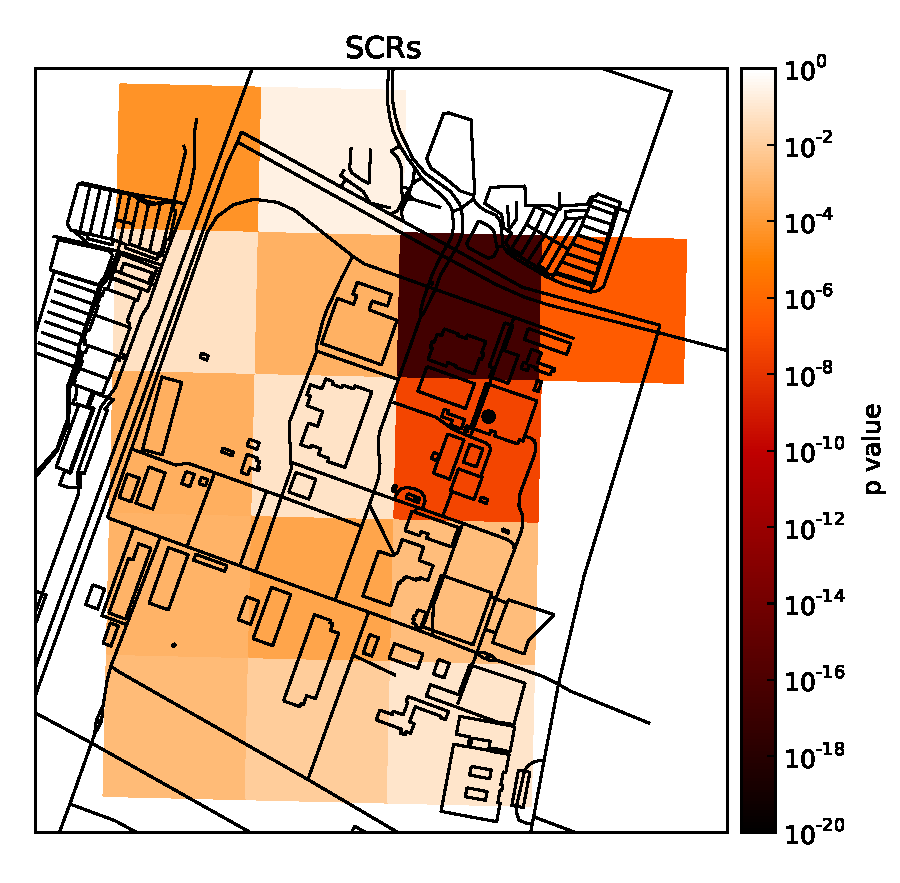
\includegraphics[width=4in]{figures/scr-injected-prc.pdf}
  \caption{Example simulated data from the Pickle Research Campus data described
    in Section~\ref{prcdata}. Here, a 650 mCi cesium-137 radioactive source has
    been injected at the location of the black dot; the resulting spectral
    anomaly is shown in dark red. The detector never traveled closer than 160
    meters to the source.}
  \label{scr-injected-prc}
\end{figure}
